%!TEX root = ../dokumentation.tex

\chapter{Couchbase (Document)} \label{ch:couchbase}
\chapterauthor{Taha Erkoc, Lara Hennes, Christian Herzgen and Ilya Suplin}

Migrating relational databases to \ac{NoSQL} databases is a problem many companies need to face when they adapt to new standards in the industry. Doing so can be a tedious process as there are many different \ac{NoSQL} databases with their own query language to choose from and developers need their time to adapt.

This is where Couchbase comes into play. It is a semi-structured, document-oriented database that saves its data in \ac{JSON} documents. With its multimodel trait and unique query language \ac{N1QL}, Couchbase is the fastest document oriented database to adapt to. This is mainly because \ac{N1QL} features the same syntax as \ac{SQL} \parencite{BigdataInsiderOnCouchbase}.

\section{History}

Couchbase was formed as a fusion between CouchOne and Membase in 2011, two companies with very different approaches to databases. CouchOne with its still known database Couch DB focuses on mobile and offline use cases to support unreliable network connections. Opposed to that, Membase works on scaling important apps and performance, by using the technical development of servers, as the system behind Zynga, a large browser game company. By fusing these two technologies, Couchbase was born and with it, the Couchbase Server System, where the service is running. Together they created a database, that is not only scalable both up and down, but also supports offline use cases \parencite{CouchOne-Membase-Fusion}.

In its early stages, Couchbase was a key-value database, but with the release of Couchbase Server 2.0 in 2012, it became the now known document-oriented database. Throughout the years, Couchbase improved their software and in 2021 released Couchbase Server 7.0, which is the current major version this chapter will discuss \parencite{CouchbaseAbout}.

\section{Architecture}

Knowledge of a database's architecture is one of the key factors to understanding its use. Couchbase offers an easy to use and implement architecture, that even beginners will understand.

\begin{figure}[H]
    \centering
    \caption{Couchbase Architecture \parencite{CouchbaseArchitecture}} \label{fig:CouchbaseArchitecture}
    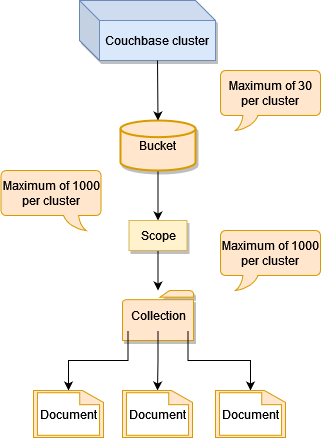
\includegraphics[width=0.5\textwidth]{images/CouchbaseArchitecture.drawio.png}
\end{figure}

This overview of a Couchbase cluster is everything one needs to get started. The \ac{JSON} documents are stored in collections, which are put into scopes. These scopes are further put into buckets, that are the top layer of storage \parencite{CouchbaseIntroduction}.

A cluster consists of one or multiple interchangeable nodes, that communicate peer-to-peer and can stand alone. One node can be any computer system running the Couchbase Server system \parencite{CouchbasePaper}.

Each node has a Cluster Manager, which is responsible for node coordination and also acts as an interface for users to administrate the cluster. Starting out with the first node, there will be four services running:

\begin{itemize}
    \item Data Service
    \item Index Service
    \item Query Service
    \item Search Service
\end{itemize}

These services can be configured across nodes, so that a cluster can consist of four nodes, with each node running one of the services. It is also possible to run the same service on multiple nodes \parencite{CouchbaseIntroduction}.

To sum up, every node in a cluster has a cluster manager and storage as seen in (fig \ref{fig:CouchbaseArchitecture}) as well as services, that can be spread across nodes. This allows Couchbase to implement \ac{MDS} to their database, that offers the opportunity for users not only to scale-up, but also scale-out their database \parencite{CouchbasePaper}.

\section{API}

Most \ac{NoSQL} databases support \acp{API}, which make administrating over \ac{HTTP} possible and easy to use.

Couchbase provides an \ac{REST} \ac{API}, that supports various functions from cluster creation to managing nodes and retrieving statistics of a database. Currently, there are thirteen different \ac{REST} \acp{API} to use, the most important ones being Nodes and Clusters \ac{API}, Buckets \ac{API}, Scopes and Collections \ac{API} and Memory and Storage \ac{API}. With these, users can create and manage their clusters and set up an entire database, configuring different buckets, collections and storage allocation. The Query Service \ac{API}, which supports \ac{N1QL} queries, and the Search Service, which provides full text searches in the database, allow users to get started with using Couchbase \parencite{CouchbaseAPI}.

There is much more functionality to explore with the rest of the different \acp{API}. They can be accessed and tested before setting up a Couchbase cluster.

\section{Advantages \& Disadvantages}

Couchbase has gained popularity in recent years due to its ability to provide high performance, scalability, and availability. However, like any technology, Couchbase has its advantages and disadvantages, which must be considered before implementing it.

One of the main advantages of Couchbase is its ability to provide high performance. Couchbase uses a distributed architecture, which allows it to distribute data across multiple nodes and process data in parallel. This results in faster data retrieval and lower latency. Additionally, Couchbase's caching mechanism, known as in-memory caching, allows it to store frequently accessed data in memory, which further enhances its performance \parencite{Couchbase.20230414, Couchbase.Review, CouchbaseArchitecturalAdvantages}.

Scalability is another advantage of Couchbase. Couchbase is designed to be horizontally scalable, which means that additional nodes can be added to the cluster to handle increased workload. This allows organizations to handle a larger number of users and transactions without compromising performance \parencite{Couchbase.20230414, Couchbase.Review, CouchbaseArchitecturalAdvantages}.

Couchbase also provides high availability by using a replication mechanism that ensures data is always available even if a node fails. In addition, Couchbase enables automatic failover, which means that if one node fails, the workload is automatically transferred to another node so that there is no downtime \parencite{Couchbase.20230414, Couchbase.Review, CouchbaseArchitecturalAdvantages}.

However, Couchbase also has some disadvantages. One of the main disadvantages is its complexity. Couchbase's distributed architecture can be difficult to set up and configure, especially for organizations without experienced database administrators. Additionally, Couchbase's licensing model can be expensive for small organizations, which may limit its adoption \parencite{CouchbaseDisadvantages, CouchbaseProsAndCons}.

Another disadvantage of Couchbase is its limited query capabilities. While Couchbase provides a \ac{SQL}-like query language, it is not as robust as traditional \ac{SQL} databases. This can make it difficult to perform complex queries and reporting \parencite{CouchbaseDisadvantages, CouchbaseCons}.

In conclusion, Couchbase has several advantages, including high performance, scalability, and availability. However, it also has some disadvantages, such as complexity and limited query capabilities. Before using Couchbase, organizations should carefully consider both sides and ensure that it aligns with their specific needs and requirements.

\section{Improvement compared to relational database design}

Couchbase's distributed architecture, flexible schema, and in-memory caching mechanism makes it an attractive alternative to \acp{RDBMS} for many use cases.

One of the biggest positive aspects of Couchbase over \acp{RDBMS} is its distributed architecture. Couchbase uses a shared-nothing architecture, which means that data is distributed across multiple nodes. This allows Couchbase to scale horizontally by adding more nodes to the cluster, which improves performance and availability. In contrast, \acp{RDBMS} typically use a shared-disk architecture, which can lead to performance bottlenecks and limited scalability \parencite{CouchbaseVsRelational, ComparingDatabases, DifferencesBetweenDatabases}.

Furthermore, Couchbase uses a flexible schema, which means that data can be stored in a variety of formats, without the need for predefined tables or columns. This allows for greater flexibility in data modeling and
and reduces the need for costly database migrations. In contrast, \acp{RDBMS} require a predefined
schema, which can be inflexible and requires significant effort to change \parencite{CouchbaseVsRelational, ComparingDatabases, DifferencesBetweenDatabases}.

Another advantage of Couchbase is its ability to handle unstructured data. Couchbase can store and process \ac{JSON} documents, which allows for greater flexibility in data modeling and reduces the need for complex joins or queries. This can be especially beneficial for applications that require complex data structures, such as e-commerce or social media platforms. \acp{RDBMS} typically require structured data, which can limit the types of data that can be stored and processed \parencite{CouchbaseVsRelational, ComparingDatabases, DifferencesBetweenDatabases}.

Lastly, Couchbase's in-memory caching mechanism allows it to store frequently accessed data in memory, which improves performance and reduces latency. This mechanism can be especially beneficial for use cases that require real-time data processing, such as online gaming or financial trading applications. \acp{RDBMS} typically do not offer in-memory caching, which can lead to slower performance and higher latency \parencite{CouchbaseVsRelational, ComparingDatabases, DifferencesBetweenDatabases}.

These advantages make Couchbase much more efficient for many use cases, particularly those that require high performance, scalability, and flexibility in data modeling.

\section{CAP Theorem}

Since the \ac{CAP} Theorem only takes a very superficial view of a system and cannot address specific aspects and features, it is difficult to place Couchbase in one of its three dimensions.

In a default single-cluster deployment, Couchbase can be classified as a \ac{CP} system, right alongside its \ac{NoSQL}-competitors MongoDB and Redis. In a single-cluster Couchbase database, consistency and partition tolerance are its most important characteristics \parencite{Ostrovsky.2015}. In case of a node failure, the Couchbase cluster will not accept writes for documents if the consistency of these documents cannot be guaranteed. This is especially useful for read and write operations on single documents.

However, in a multi-cluster deployment, Couchbase uses \ac{XDCR} to achieve availability in favor of consistency \parencite{CAPXDCR.2014}.

\ac{XDCR} allows data to be replicated across clusters. The data contained inside a source bucket is replicated to a target bucket, which primarily serves as a backup. This can be done either uni- or bidirectionally, with the latter replicating data inside the target bucket to the source bucket, thus allowing both buckets to be used to serve data. These clusters can be located in totally different data centers, which enables faster access for users and applications that are in remote locations \parencite{XDCR.20230402}.

In case of a node failure, the data located in the replicated target bucket can be used to read/write, guaranteeing high availability even though the data might not be consistent. This is called \textit{eventual consistency} \parencite{DonPintoPrincipalProductManager.2014}. All writes to the database are done asynchronously across the nodes inside the cluster, which means that different nodes might have different versions of the same data at any given time. Eventually, all nodes will converge into the same state, however the time it takes to achieve convergence can depend on many factors such as network latency, load and frequency of updates. \ac{XDCR} provides several conflict resolution mechanisms to solve problems that can arise when changes are made to the same document on multiple clusters.

\begin{figure}[H]
    \centering
    \caption{Bidirectional \ac{XDCR} \parencite{XDCR.20230402}}
    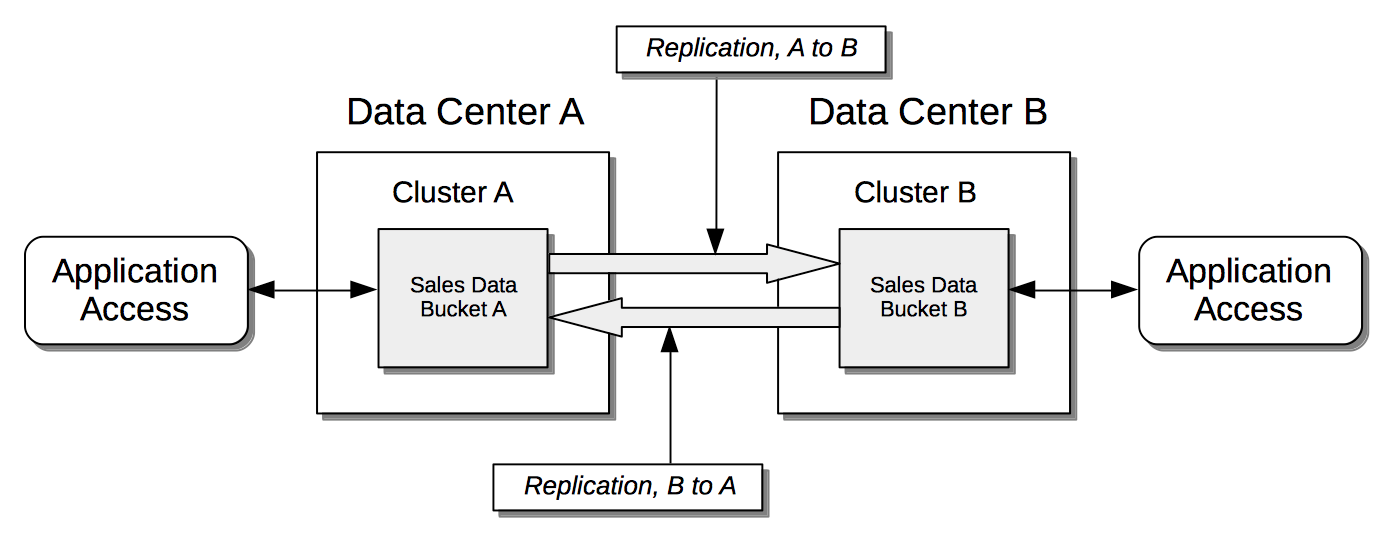
\includegraphics[width=0.7\textwidth]{images/bidirectional-xdcr.png}
    \label{fig:BidiXDCR}
\end{figure}

To achieve partition tolerance, Couchbase uses its \textit{Auto Failover} feature, where nodes can be failed over automatically if they become unresponsive, so the service remains available and responsive for clients even in times of network failures \parencite{Autofailover.20230402}.

As one can see, applying the \ac{CAP} theorem to Couchbase is rather difficult since it heavily depends on its deployment method. In summary, Couchbase can be used as both a \ac{CP} and \ac{AP} system, with single cluster systems being configured as \ac{CP} and multi cluster systems configured as an \ac{AP} system. Couchbase provides mechanisms for enforcing both consistency and availability while handling network partitions and failures, so users can have a seamless experience using it.

\section{Fields of Application}

With its highly scalable and flexible nature, Couchbase has a wide range of applications in various industries. Its high-performance and features make Couchbase a good choice for web and mobile applications as well as e-commerce, finance, healthcare and gaming \parencite{Couchbase.20230329}.

In e-commerce applications, which is the most common use case for Couchbase, it is used to store and manage user profiles, product catalogs and transactional data. It allows companies to deliver personalized shopping experiences with real-time inventory updates to their customers.

Ad tech companies use Couchbase to store and manage large amounts of data such as user profiles, ad impressions and clickstream data. It can handle high volumes of data and provides real time analytics, thus enabling ad tech companies to deliver personalized ads to their customers.

In healthcare, Couchbase is used to store and manage patient data. With its robust security and compliance features, it allows healthcare organizations to protect sensitive patient information.

Couchbase can work with large amounts of unstructured data and, since its schema is not fixed, can easily adapt to changing requirements. Its distributed architecture also makes it efficient in use cases regarding Internet of Things or real time Big Data \parencite{StudentCouchbase.}.

Especially companies, that want to have the benefits of \ac{NoSQL} databases, but have difficulties migrating their relational database management system, use Couchbase since its \ac{N1QL} query language is very similar to the well-known \ac{SQL} language.

Overall, Couchbase is a highly versatile and scalable database that can be used in many different industries. Its fast data access, scalability and features make it a valuable tool for modern applications. Couchbase is used in many different industries by various companies such as PayPal, LinkedIn, Emirates and many more.


\section{Installation and setup of database}

\subsection{Installation on Windows}

To install Couchbase on Windows, there are certain prerequisites which need to be met before the installation. The user needs to have Windows 10 Universal CRT installed, they need admin rights and no previous version of Couchbase should be installed. It is important to delete traces of previous installations before the new installation. The user can then download the MSI file on the Couchbase website. After the download, it can be easily installed, by executing the downloaded installer with admin rights \parencite{Couchbase.20230318}.

\subsection{Installation with Docker}

If the user wants to have multiple nodes, or does not have a clean system, we recommend installing Couchbase in a Docker Container. Couchbase has an official Docker image, which can be found in the Docker Hub. With the following command, the Docker Container can be started on the machine. This command is best for a single instance of Couchbase. With the ``-p'' flag the port mappings to the machine can be specified.

\begin{lstlisting}
docker run -d --name db -p 8091-8096:8091-8096 -p 11210-11211:11210-11211 couchbase
\end{lstlisting}

If the user wants to run multiple instances of Couchbase on the same machine in Docker Containers, they should leave out the ``-p'' flag and change the ``-name'' each time. To then access the containers, they have to look up the \ac{IP} address of each container \parencite{Couchbase.20230318b}.

\subsection{Setup}
One way of setting up Couchbase is through the \ac{UI}. By default, the Couchbase Web Console is running on port 8091. To access it, the user should open ``http://<machine-ip-address>:8091/'' in a browser of their choice. When opening the \ac{UI}, the user has the choice to either add a node to an existing cluster or set up a new cluster. When setting up a new cluster, the user needs to create an admin user can then configure the settings for the cluster. After these steps, the node is ready for use \parencite{Couchbase.20230401}.

It is also possible to set up the node through the \ac{CLI} or the \ac{REST} \ac{API}, however this process will not be explained in this e-book.


\section{Example}

In the following section, an example for a relational database taken from the Database I lecture is transformed to a document based model. The different architecture, \ac{N1QL} for the population of the database and the Couchbase query editor are shown.

\subsection{Architecture}

The architecture for the \ac{SQL} database has multiple tables, with some tables to store the relations. There is the ``Produkt'' and the ``Zusatzstoff'' table which are connected through the``ProduktEnthaeltZusatzstoff'' table. In the transformation to Couchbase there is a product collection with records where each record references the IDs of the corresponding records in the zusatzstoff collection in an array.

\begin{figure}[H]
    \centering
    \caption{Architecture Examples}
    \begin{subfigure}{0.48\textwidth}
        \centering
        \caption{Architecture Example with \ac{SQL}}
        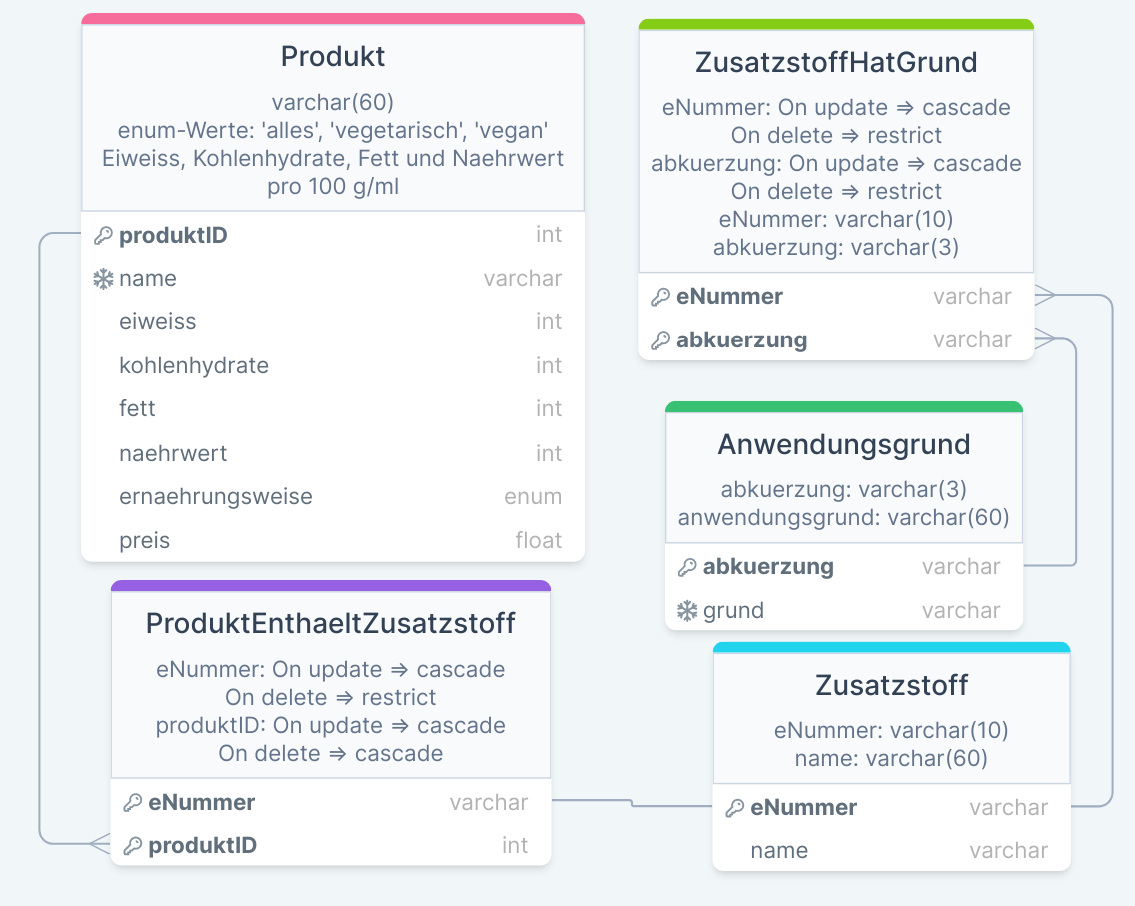
\includegraphics[width=1\textwidth]{images/Architecture_Example_SQL.png} % first figure itself
    \end{subfigure}\hfill
    \begin{subfigure}{0.48\textwidth}
        \centering
        \caption{Architecture Example with Couchbase}
        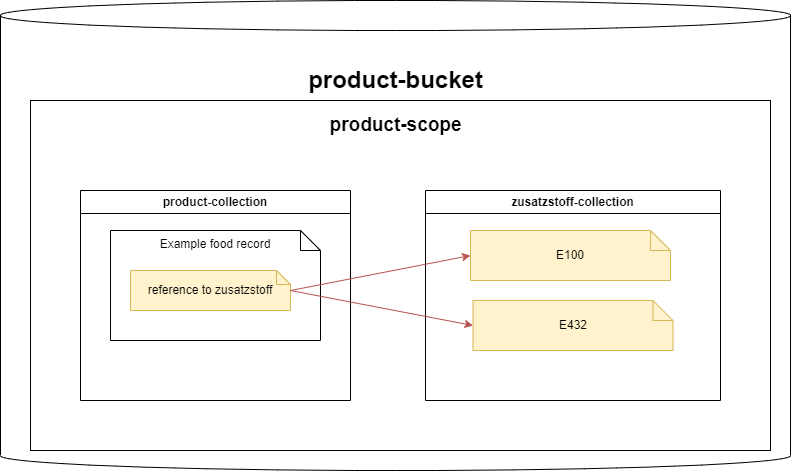
\includegraphics[width=1\textwidth]{images/Architecture_Example_Couchbase.png} % second figure itself
    \end{subfigure}
\end{figure}

\subsection{N1QL}

If the user wants to populate their database, they can do so by using queries. These queries have to be written in \ac{N1QL}, which is very similar to \ac{SQL}. Based on the Couchbase Architecture, first a bucket and a scope have to be created. The bucket can not be created through a query and has to be created in the \ac{UI} or \ac{CLI}. The scope can then be created in the bucket. After that, it is possible to create the collections in the scope. In the end, an index needs to be created on the collection, as otherwise the user will not be able to execute a select statement on the collection.

\begin{lstlisting}
CREATE SCOPE productBucket.productScope IF NOT EXISTS
CREATE COLLECTION productBucket.productScope.product IF NOT EXISTS
CREATE COLLECTION productBucket.productScope.zusatzstoff IF NOT EXISTS
// if context is set in query editor
Alternative with set context in query editor: 
CREATE COLLECTION zusatzstoff IF NOT EXISTS
// creation of index
CREATE PRIMARY INDEX zusatzstoff_idx ON zusatzstoff
\end{lstlisting}

To insert a document into the database, the upsert functionality can be used. This means, the document with the specified ID will be created if it does not exist, or if it already exists it will be updated. It is possible to upsert multiple entries at once. With the "returning" part of the statement, all the added documents will be returned. The ``*'' stands for all information in the document, the ``META().id'' returns the document ID as the ID is not in the document its self \parencite{Couchbase.20230314}.

\begin{lstlisting}
UPSERT INTO zusatzstoff (KEY, VALUE)
VALUES ("E100", {"name ": "Kurkumin", "gruende": ["Farbstoff"]}),
VALUES ("E150", {"name ": "Zuckerkuloer", "gruende ": ["Farbstoff", "Suessungsmittel"]})
RETURNING META().id, *;
\end{lstlisting}

``SELECT'' works very similar as it works in \ac{SQL}. It is possible to specify conditions with the ``WHERE'' clause. A functionality, that has been added, is ``MISSING''. Because Couchbase does not enforce a schema, some documents can have missing attributes. These can be used in the statement for filtering. Joins between collections are possible as well, additionally the ``NEST'' clause has been introduced which can be used for arrays in a document \parencite{Couchbase.20230314b}.

\begin{lstlisting}
SELECT p.name, p.preis FROM product AS p WHERE preis < 2
SELECT p.name FROM product AS p WHERE eiweiss IS MISSING
\end{lstlisting}

\subsection{Query Editor}

\begin{figure}[H]
    \centering
    \caption{Couchbase Query Tool}
    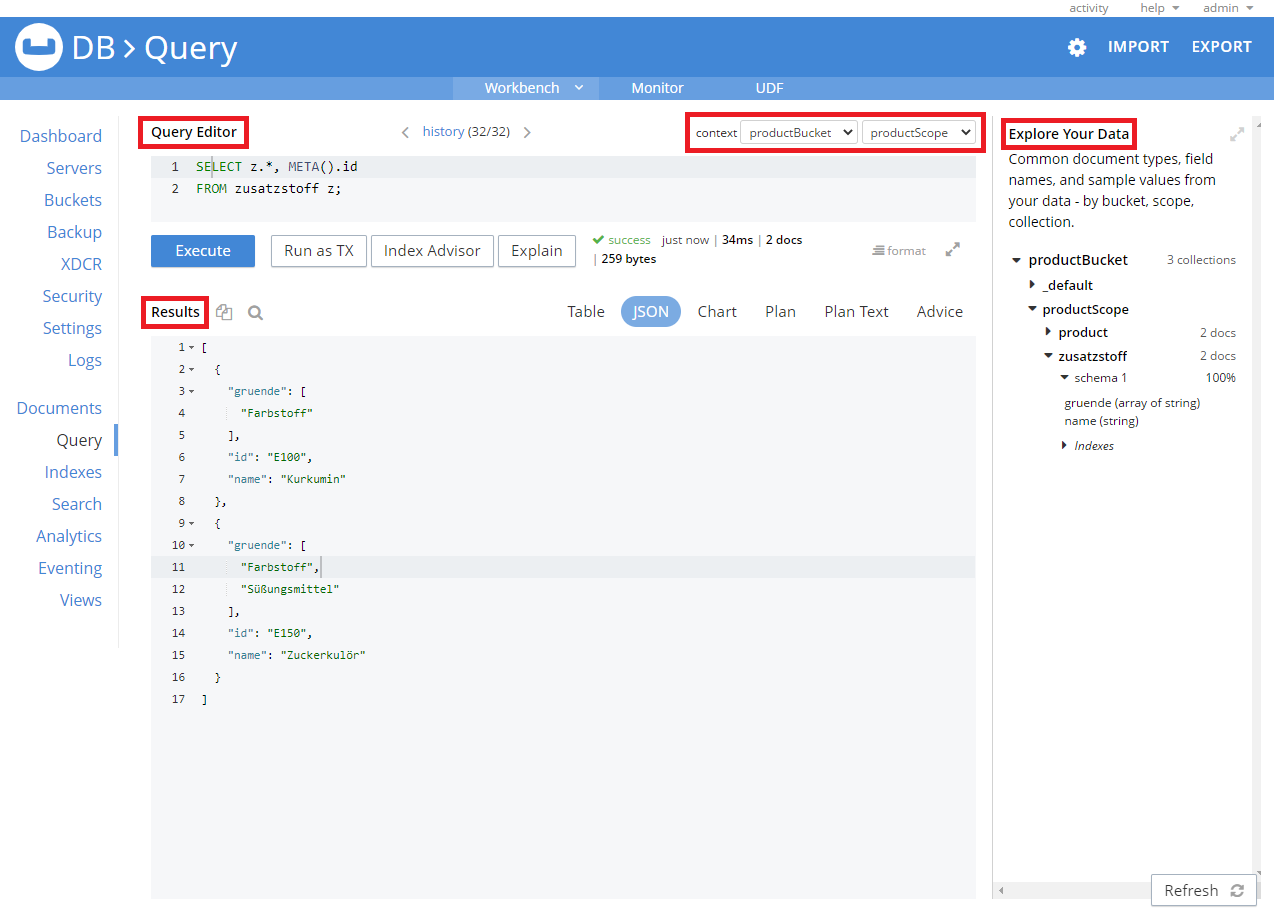
\includegraphics[width=\textwidth]{images/Query_Tool_Couchbase_marked.png}
    \label{fig:CouchbaseQueryTool}
\end{figure}

Couchbase offers a Query Editor in its \ac{UI}. This tool can be used to execute queries on the database. The query has to be written in \ac{N1QL} in the editor text field. The "Execute"-button can then be used to carry out the query.

In the "Results" part, the result to the query is shown. By default, a \ac{JSON} is returned, but other formats can also be chosen.

The context drop-down menu can be used by the user to set the context where a query should be executed. The user can select the bucket and after selecting the bucket they can choose the scope. By doing this, the user eliminates the necessity to specify the path for the collections.

The "Explore Your Data" section displays all the collections in the different buckets and scopes. It shows the number of docs, and the different schemes of the documents inside a collection are displayed.

The Query Editor saves all the executed queries in a history. The history is downloadable and can also be re-uploaded so the queries can be reused \parencite{Couchbase.20230325}.


\section{Recommendation \& Conclusion}

Couchbase offers advantages of CouchDB and Membase, optimized for concurrent read and write operations and supports \ac{JSON} documents. Its \ac{SQL}-like query language \ac{N1QL} simplifies migration of relational databases, and it uses clusters and buckets for data storage. Couchbase's classification is challenging because the \ac{CAP} theorem is superficial and cannot address specific aspects. Consistency and partition tolerance are most important in a single-cluster system, while the \ac{XDCR} feature is used for availability at the cost of consistency in multi-cluster systems.

It is difficult to enforce a schema in Couchbase, meaning it is better suited for a more flexible use case. We recommend using it for migrating \ac{SQL} to \ac{NoSQL} databases, as developers can easily adapt to the query language. Especially modern web and mobile applications can benefit from Couchbases scalability and performance. While not as popular as its direct competitor MongoDB, Couchbase should not be underestimated, as it actually outperforms MongoDB in many areas such as scalability and performance.
